\chapter{Introduction}
\thispagestyle{empty}
\label{chap:introduction}

\emph{This first chapter introduces the reader to concepts such as gene, chromosome 
and DNA all the way up to Multiple QTL mapping (MQM) and Genome Wide Association Studies 
(GWAS). }

\null
\vfill
\newpage

\section{From pea plants to 'Big Data'}
Since the first genetic theories on the inheritance of phenotypes in pea plants were published by 
Gregor Mendel in 1865, the ongoing interest in the field has now resulted in an unprecedented stream 
of data to study Biology. The knowledge gain from Genetics research is huge as it has revealed how 
complex Biology actually is. 

Genetics research has shown how the activity of DNA is regulated by signals from all molecular levels, 
i.e. the genome, transcriptome, proteome, and metabolome. All these levels interact, and they are also 
modified by signals from the environment. Adding to the complexity, every level in the genetic paradigm 
has its own chemistry, functionality, and research technologies (See table \ref{tbl:overview}). Systems 
genetics is the research field in which we consider all these levels and interpret them together, within 
the context of DNA. Systems genetics aims to find the DNA variants underlying the variation that is 
seen on the higher molecular levels, all the way up to the phenotypes, for example seed quality in plants, 
and Crohn's disease in humans. 

The research fields of Genetics and Bioinformatics have been intertwined for several decades. Since the 
1980s it has become impossible to analyse data without using some form of computational assistance. This 
forces geneticists either to become 'computer savvy' or to collaborate with bioinformaticians. In practice, 
Genetics research has evolved into an interdisciplinary research domain. This thesis enters the field from 
the Bioinformatics perspective.

The ongoing stream of data that is being produced in the field of Systems genetics, poses several 
challenges to bioinformaticians. Data storage, computation on the data, and visualising the results, 
becomes increasingly harder when data sizes increase. For example, a clinician who has to deal with 
gigabytes of data while diagnosing a patient, requires access to good software. On a research level, 
understanding how a system works and reacts to different environments, allows modification of the system 
to better suit our needs or environmental requirements. The expected impact of such knowledge about DNA 
variation is to optimise  the breeding of livestock and crops, explore the genetic basis of human diseases, 
improved production of chemicals, and so forth. The use of computational tools in understanding how 
genetics and the environment intertwine is thus central to the field of Systems genetics and forms the 
basis how to deal with the large amounts of phenotype and genotype data. How we transform such data into 
usable knowledge is the main theme of this thesis.

\begin{table}[h]
  \centering
  {\footnotesize
  \begin{tabular}{ | c | l | l | }
    \hline
    {\bf Molecular level} & {\bf Molecule} & {\bf Technology}\\
    \hline
    \hline
\rowcolor{gray!35}    Genome          & DNA                & RFLP \cite{Lander:1986} \\
\rowcolor{gray!35}    Genome          & DNA                & SNP chips \cite{Hacia:1999} \\
\rowcolor{gray!35}    Genome          & DNA                & DNA sequencing \cite{Mardis:2008} \\
    \hline
    EpiGenome       & DNA methylation    & Bisulfite sequencing \cite{Hayatsu:2007} \\
    EpiGenome       & DNA methylation    & ChIP-on-chip \cite{Collas:2010} \\
    EpiGenome       & DNA methylation    & ChIP-Seq \cite{Park:2009} \\
    \hline
    \hline
\rowcolor{gray!35}    Transcriptome   & RNA          & Microarray \cite{Lashkari:1997}, Tiling array \cite{Lee:2013} \\
\rowcolor{gray!35}    Transcriptome   & RNA          & RNA-Seq \cite{Wang:2009}\\
    \hline
    Proteome        & Proteins     & 2D gel electrophoresis \cite{O'Farrell:1975}\\
    Proteome        & Proteins     & Mass Spectometry \cite{Deshaies:2001}\\
    Proteome        & Proteins     & Antibody protein chip \cite{Fasolo:2009} \\
    \hline
\rowcolor{gray!35}    Metabolome      & Metabolites  & Mass Spectometry \cite{Aebersold:2003} \\
\rowcolor{gray!35}    Metabolome      & Metabolites  & Nuclear magnetic resonance \cite{Espina:2009} \\
    \hline
  \end{tabular}
  }
  \caption[Overview]{Overview of current technologies to interrogate the molecular basis for life.}
    \label{tbl:overview}
\end{table}

Currently new data types are coming in more often than before. Previously geneticists dealt with mostly 
classical phenotypes and a limited number of genetic markers. Now we are able to map 1000s of traits onto 
millions of markers, creating not only more data, but also a more diverse kind of biological data. These 
new data also need to be considered when analysing and interpreting the outcome in terms of clinical and 
societal relevance. To merge all these inputs and give algorithms a unified view on such diverse data, 
requires generic data modelling, and generators that use these models to create de-novo (web)-infrastructure, 
such as clusters, clouds and multi-core machines. 

The phenomenon of larger sample sizes, more data collection, and more intense computations, is a natural 
consequence of the data driven research which has increasingly become the focus of Systems genetics. Data 
driven research has caused the issue that we now call 'Big Data'. Making sense of this Big Data is increasingly 
difficult as it becomes harder to find clinical and societal relevant conclusions, while requiring ever 
larger computer facilities. This leads to increased societal costs, most notable in healthcare and industry. 
In the context of all these developments, it is important to consider more efficient usage of available 
resources, and avoid duplicate work effort. To contribute to this challenge we formed the following central 
question in this thesis:

How can computational bioinformatics help solving current 'Big Data' issues in Systems genetics?

\section{Approaches}

Recent developments in the computational infrastructure have created many new possibilities to deal with 
complex data in a powerful way. The impact of these developments is that all kinds of genetic concepts can 
now be tested. For example, 20 years ago the concept of Multiple QTL Mapping (MQM) was developed. This technique 
aims to compare all genetic markers to each other. At the time when MQM was conceptualised, it was computational 
very demanding. Because of the current increase of computational power, we are able to revisit MQM's methodological 
challenges and demonstrate that using smarter ways of computation will allow us to solve research questions and 
do this in reasonable time. 

QTL mapping associates phenotype variation with genetic variation using appropriate statistical methods, such as 
t-tests, anova, and generalised linear models. MQM is a two-step procedure. First, it uses generalised linear models 
and backward selection of genetic cofactors to model the number of genetic factors underlying the phenotypes. In 
the second step, it uses the optimal model for QTL detection conditional to the selected cofactors. MQM is a superior 
technique compared to other methods for QTL mapping, as it allows detection of QTL in repulsion phase and performs 
with higher statistical power to detect phenotype to genotype associations. These advantageous characteristics 
are key to our decision to reintroduce the MQM algorithms into the Bioinformatics toolbox.

The Bioinformatics toolbox R/qtl \cite{Broman:2003, Arends:2010} is an open-source toolbox for mapping QTLs in inbred 
animals. It provides many QTL mapping routines and allows researchers to easily switch between statistical approaches, 
or test new approaches for QTL detection. Furthermore, it comes with a large user base and is de facto standard in 
the mouse QTL mapping community.

High throughput phenotyping provides us with data on thousands of phenotypes. Some of these phenotypes can be used 
as genetic marker because they show a major QTL effect. This leads to a situation in which we have a low quality genetic 
map and an abundance of phenotypes which could be used to improve the map quality. This knowledge, combined with a 
lack of good genetic map creation software in the R/qtl package, has fuelled the development of the sensitive algorithm 
Pheno2Geno. It uses mixture modelling, combined with a sensitive pre-selection approach. This results in faster 
genetic map creation as compared to other methods, and is the main reason for our ambition to add Pheno2Geno to R/qtl. 

QTL interactions are a novel area of interest in Systems genetics. For example, in recent years several papers were 
published on cell type or sex specificity of QTLs. Detection of these cell type specific QTLs has proven to be extremely 
difficult because it requires large sample sizes.  Meta-analysis, where we combine the samples from separate studies 
to improve power, is a prerequisite when studying cell type specific expression-QTLs (eQTLs). We noticed a lack of 
good software to meta-analyse these cell type specific QTLs in a genome wide setting. Furthermore, since cell type specific 
eQTL analysis is comparable to analysis that uses multiple environments, we propose to conceptualise cell abundance 
similar to an environment in which a QTL can be present or absent. Therefore, to consider such interactions, our toolbox 
also needs to be adjusted to support meta-analysis on genetical genomics experiments in which these QTL x Environment 
interactions are included.

Considering these methodological Big Data issues in Systems genetics, the following sub-questions were formulated to 
guide the research: 

1. Whether and how can QTL be used in high-throughput trait data to computationally generate high (or higher) numbers of genetic markers to more accurately fingerprint samples? 

2. Whether and how can software for QTL analysis, in particular MQM for complex traits, be scaled up to cope with dense fingerprint/marker information and high-throughput trait data?

3. Design software infrastructure for storage of, and computation on high-throughput fingerprint/marker and trait data.

4. Which benefits of research questions 1-3 can be demonstrated on real high-throughput data, and which (Systems) biological insights does this reveal? 

\section{The first genetic theories (1800-1930)}
As this research project approaches 'old' genetic theories with new Bioinformatics tools, it is relevant to place 
them in their historic context. The research field of genetics is relatively old, as it is founded when Gregor 
Mendel publishes his work on the inheritance of phenotypes in pea plants. His work, described in 'Versuche über 
Pflanzen-Hybriden' in 1865-1866 \cite{Mendel:1866}, gives us Mendel's Laws of Inheritance. He observed that crossing 
two plants with different flower colours leads to an offspring population with predictable colour ratios. He 
postulated the idea of heredity units and stated that each individual carries two of these, which results in a 
single phenotype. Each heritable unit is received from one of the parents, but which one is passed on to the 
offspring is random. Mendel formulated this principle as First Law on Segregation: if two units are not equal, 
a dominant unit (colour 1) overrules another unit (colour 2 - recessive). 

Additional to studying colour, Mendel also studied other phenotypes in the pea plants besides colour. Now we know 
that Mendel was fortunate to select phenotypes which are caused by a single gene and are inherited independently. 
Mendel also observed this phenomenon of independent inheritance when comparing the inheritance of multiple 
phenotypes. He concluded that a unit of inheritance is passed from parent to offspring in an independent fashion, 
that is, independent  from other phenotypes that are inherited. This principle is known as Mendel's Second Law 
on Independent Assortment.

The relevance of Mendel's inferences was not fully recognised until 30 years later, when his work was rediscovered 
by Hugo de Vries, Carl Correns, and Erich von Tschermak. They (re)defined the rules for Mendelian Genetics \cite{deVries:1889}. 
In doing so, they provided biologists for the first time with a mathematical framework to study heritability of 
phenotypes caused by a single genetic unit.

Twenty years after the rediscovery of Mendel's Laws, careful observations of Thomas Hunt Morgan introduced in 1913 
an addition to Mendel's theoretical work. He observed that some phenotypes in his Drosophila melanogaster mutant 
flies are inherited together. This is in conflict with Mendel's Laws, stating independent inheritance of genetic 
units. Morgan called this phenomenon genetic linkage. A specific situation arises when phenotypes are linked to 
the sex of the animal. This is called sex based inheritance \cite{Morgan:1915, Morgan:1916}.

Mendel worked on plants, while Morgan worked on fruit flies. Although the genetic basics are very similar, the sex 
linked inheritance is not observed in most plants as they are usually male and female at the same time. Currently 
four plant families have been discovered that developed sex chromosomes acting similar to the sex chromosomes in 
animals \cite{Ming:2007}. Interestingly, these phenotypes do not follow Mendel's Second Law, as the traits are not 
inherited independently, but are linked to the sex phenotype. 

The concept of genetic linkage is commonly explained as beads on a string, in which multiple genetic units are 
linked together.  Two beads close together are tightly linked and almost always inherited together. In contrast, 
two beads that are far apart are less linked and can be separated by meiosis. Different strands are inherited 
independently, and thus allow Mendelian inheritance by two beads on two different strings. 

Sturtevant, one of Morgan's students, used his mentor's linkage theory between phenotypes as a measure of distance 
between units of inheritance. He created the first genetic map of Drosophila Melanogaster in 1916, 40 years before 
the discovery of the DNA molecule \cite{Morgan:1916}, and at a time when molecular mechanisms were still unknown. 
Sturtevant's genetic map, based on phenotypes, was used to study Genetics based on careful observation of the 
segregation of phenotypes in large populations of flies, and then determining the distance between the units of 
inheritance relative to other phenotypes. Observations showed that sometimes the link between two phenotypes is 
broken. The amount of times this is observed in a population, is taken as a measurement of distance between the 
two phenotypes. For example, when we have measured 200 phenotypes in crosses, we can estimate which belong together 
on the same chromosome, as these are the ones which are found together more often than randomly expected. Further 
exploration of the data can indicate the order of the phenotypes on the map.

Intermezzo - The same method to measure distances is nowadays used to construct genetic maps on phenotypes in Pheno2Geno. 
It differs from methods using genotypes, i.e. SNP chips, as they require DNA sequencing data. Such methods are more 
expensive because first the phenotypes are measured, followed by the genotypes. Pheno2Geno applies data of measurements 
of distance between phenotypes to subsequently define the genotypes, without a second measure.  

In 1918 Ronald A. Fisher published a paper entitled 'The Correlation Between Relatives on the Supposition of 
Mendelian Inheritance'. The paper demonstrates that a large number of small effects from discrete genetic 
units eventually add up to the continuous phenotypes observed \cite{Fisher:1918}. Fisher proposed to unify all 
phenotypes, discrete and continuous, in one model. Mendel's theories could only explain dichotomous phenotypes, 
e.g. yellow versus green, but the phenotypes that were most interesting to researchers, are continuous. As 
Mendel's theory did not apply to these, his work was ignored in favour of other theories. Fisher developed 
mathematical approaches to explain continuous phenotypes, such as human stature, and showed that they follow 
Mendel's Laws. He proposed that geneticists had to search for a number of small effect loci. Summation of 
these small dichotomous effects from many genetic units on a population scale would add up to the observed 
normal distribution. (This theory was only proven after Watson \& Crick and the discovery of DNA and genes).

With this observation we move to the next section, in which a book by R. Fischer again plays a major role in 
the development of population genetics.

\section{DNA and QTLs (1930-1990)}

In 1930, Fisher published the book 'The Genetical Theory of Natural Selection' \cite{Fisher:1930}. Fisher describes 
how Mendelian genetics is consistent with the idea of evolution by natural selection. His reasoning turned out 
to remove one of the last barriers for large scale adoption of Mendel's theories in Biology. The subsequent discovery 
of DNA as the carrier of heritability by Avery, MacLeod and McCarty in 1944 \cite{Avery:1944}, and the discovery of 
its structure by Watson and Crick in 1953 \cite{Watson:1953}, revealed the long sought-after molecular basis for Genetics. 

After the discovery of restriction enzymes by Luria and Human \cite{Luria:1952} it was possible to cut and paste pieces 
of DNA. This allowed to experimentally work with DNA and investigate the different (lengths of) fragments produced, 
create new combinations of known DNA, and even novel DNA sequences to study the heritability of phenotypes. In 1970 
the first techniques were developed to sequence DNA. The first approach used two-dimensional chromatography, and was 
followed by fluorescence based sequencing methods \cite{Pettersson:2009}.

\begin{wrapfigure}{r}{0.5\textwidth}
  \centering
  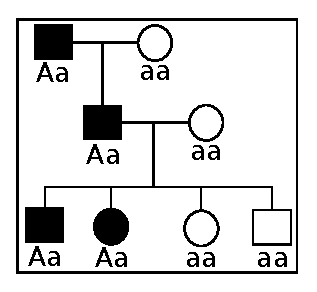
\includegraphics[width=0.4\textwidth]{eps/image_1_2.eps}
  \caption[Example of pedigree based linkage analysis.]
    {Example of a hypothetical pedigree on which linkage analysis can be performed. Here we show a 
    hypothetical pedigree of individuals within a family (2 generations), squares represent 
    male individuals while circle are females. The phenotype is shown encoded by the fill 
    color of the shape (Black = affected, White = not affected).  In this example pedigree, 
    the "A" allele segregates with the disease. It is shared identical-by-descent in all 
    affected individuals. }
    \label{fig:pedigree}
\end{wrapfigure}

By the end of the 1980s everything was there for the next big step in Genetics. Three papers were published which detailed 
the use of Restriction fragment length polymorphism (RFLP) linkage maps to localise genes responsible for variation in 
quantitative phenotypes. These three papers by David Botstein and Eric Lander \cite{Lander:1986, Lander:1987, Lander:1989} 
form the basis for modern day linkage analysis and genome wide association studies. This allowed, for the first time in 
history, the direct association of DNA with its effect on a phenotype. 

These tools are used by geneticists and bioinformaticians to identify the region of DNA underlying phenotypes or diseases 
(if any). These regions are in themselves already interesting because they provide targets to optimise the phenotype (e.g. 
when improving plant yield), or for developing therapies/drugs for human diseases. Two methods of QTL analysis are applied 
in searching  DNA regions, i.e. linkage analysis and association analysis. 

\emph{Linkage analysis} is the DNA technology to trace parents and offspring/children. It is used to build so called genetic 
family trees or pedigrees (See fig. \ref{fig:pedigree}) in which segregation of a phenotype (for example a disease) is 
displayed. When we find a genetic region that co-segregates with the disease, we can assume the DNA and the disease are 
linked, allowing assessment of the strength of the observed linkage \cite{Rosyara:2009}. When experimental crosses derived 
from inbred parents are used, the need to build up complex pedigrees is avoided, while retaining the advantage of being able 
to trace back the DNA to the founder strains. Inbred populations also provide high statistical power at the cost of reduced 
resolution for QTL mapping \cite{Jansen:2001a}. This reduced resolution is caused by the lack of recombination in small 
populations (20 to 1000 individuals). 

\begin{wrapfigure}{r}{0.5\textwidth}
  \centering
  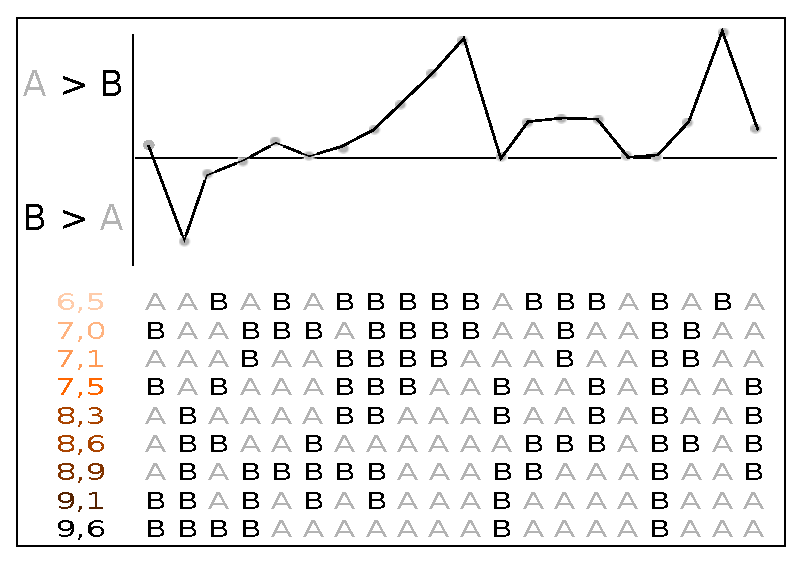
\includegraphics[width=0.5\textwidth]{eps/image_1_1}
  \caption[Effect scan across the genome.]
    {An example of how effect scans are performed using a single phenotype measured on 9 individuals (colored numbers)
    and genotypes represented by rows in the matrix (A or B). 20 markers (columns) were assessed: A and B are genetic 
    variants obtained from either parental or maternal line. }
    \label{fig:effectscan}
\end{wrapfigure}

An example of a basic effect scan using linkage analysis is shown in Figure \ref{fig:effectscan} At each marker the mean of 
the phenotype for AA and BB is calculated, and the difference is plotted per marker. This gives an initial indication which 
markers may be relevant biomarkers for the phenotype of interest.

\emph{Association analysis} can be applied in outbred, or natural populations when tracking the origin of the DNA is difficult 
or impossible. Molecular markers still allow to find information about the underlying DNA. We can use e.g. single nucleotide 
polymorphisms (SNPs) to associate a phenotype with the genetic marker \cite{Mehta:2013} The advantage of this approach is that 
the resolution is very high (around 200 - 300 kb in humans \cite{HapMap:2005}) because outbred populations have a high number of 
recombinations, as compared to inbred populations. At the down side is that the large number of markers reduces the statistical 
power to detect effects as the result of multiple testing. Heritable phenotypes can be mapped to genomic locations using a 
combination of DNA restriction enzymes, Mendel's inheritance laws, and Hunt's linkage theory. Together these methodologies and 
theories provide the experimental and statistical background to analyse heritability in any population.

Linkage analysis and association analysis, both developed in the 1980s, are still the foundation of population genetics research. 
More sophisticated tools and algorithms have been developed and implemented, but the basic theoretical concepts are the same. 
Some of these more advanced methods are discussed in the next section to sketch a background for the work presented in this 
thesis. 

\section{From phenotypes to genetical omics and GWAS (1990-2010)}

The basis of an observed phenotype expression is often more complex than a single causative gene \cite{Sinha:2006, 
West:2007}. To model these more complex interactions between multiple regulators of gene expression requires extension of 
the basic model for QTL mapping. Extending the model is done by incorporating sources of variation as co-factors. This 
allows us to associate/partition the observed variance to either environmental factors (E) or genetic loci (G). The method 
is to include additional genetic components into the model, and then scan for QTLs conditional on these other genetic effects. 
This is the basic principle of Multiple QTL Mapping (MQM). MQM belongs to a family of QTL mapping methods, that includes 
Haley-Knott regression \cite{Haley:1992} and composite interval mapping (CIM) \cite{Zeng:1994}. MQM combines the strengths 
of generalised linear model regression with those of interval mapping \cite{Jansen:1993, Jansen:1994b}.

During the first years of QTL mapping, the genetic maps were of poor quality, with a lot of missing marker data and large 
gaps between markers. As a solution to this problem interval mapping was developed. Interval mapping uses prior knowledge 
about linkage in inbred populations to map QTLs between two genetic markers. Hidden Markov models (HMMs) are used to estimate 
the unobserved genotypes in the population based on the surrounding genotype observations, thereby improving the QTL 
mapping resolution \cite{Jansen:1993, Zeng:1994}.

Genetical genomics is the concept that deals with endophenotypes (RNA, protein and metabolite abundance) as if they were 
common phenotypes. They are mapped in bulk to the genome, in a way similar to classical phenotypes \cite{Jansen:2001a}. 
Natural occurring variation and new omics tools allow us to track variation from the genotype all the way up to the classical 
phenotypes (see Table \ref{tbl:overview} for a short overview of methods). Tracing the effects of variation from genome 
to phenotype allows Genetics to go from individual QTLs to a system-wide approach of analysing QTLs at all known molecular 
levels. This approach is called Systems genetics \cite{Threadgill:2006, Nadeau:2011}

Studies in model organisms have shown high heritability's for endophenotypes, such as gene expression, making these phenotypes 
ideal targets for QTL mapping \cite{Brem:2002, Yvert:2003, Morley:2004}. In 2003 R/qtl was developed to provide reference 
implementations for QTL mapping. R/qtl is an extensible, interactive Software/R package to map quantitative trait loci (QTL) 
in experimental crosses. It is implemented as an add-on package for the freely available and widely used statistical 
language/software R \cite{R:2009} The main focus of R/qtl is to provide the mouse community with different QTL mapping 
methodologies, and allow to deal with the aberrant segregation X chromosome. Furthermore it supports different types of 
inbred populations such as backcross (BC), F2, Recombinant inbred lines (RIL) and 4-way RILs \cite{Broman:2003}.

When mapping gene expression or protein abundance current knowledge of protein and DNA sequence allows us to locate their 
template on the genome. If QTL mapping resolution is high enough, we can even distinguish between traits mapping in the 
proximity of their respective gene (cis-eQTL) or to other regions in the genome (trans-eQTL). This information can be summarised 
into so called cis-trans plots, where the X-axis is the location of the eQTL and the Y-axis the genetic location of the trait. 
Often so called trans-bands are observed, hotspots of many trans- eQTL mapping to a common region in the genome \cite{Breitling:2008a}. 
These are used to infer biological meaning and reconstruct co-expression and/or co-regulatory networks.

In the last decade Genome Wide Association Studies (GWAS) have identified thousands of genetic variants that are associated 
with human disease \cite{Hindorff:2009}. For reliable results GWAS needs a large cohort of genotyped and phenotyped individuals. 
Large consortia are working together to gather large amounts of human expression data from many different tissues. These data 
are then used in meta-analysis leading to eQTL GWA studies with even larger sizes (5000+ individuals) \cite{Lude:2011}, leading 
to more reliable results and enabling discovery of new modifiers of human gene expression. It is now recognised that many factors, 
such as effects on intermediate molecular phenotypes, influence the relationship between genotype and the eventual development 
of disease. It has also been observation that many of the disease predisposing variants are non-coding, which suggests that 
these variants have a regulatory function. Furthermore it has been shown that many disease predisposing variants (e.g. single 
nucleotide polymorphisms (SNPs)) affect the expression of nearby genes (i.e. cis-eQTLs) \cite{Zeller:2010, Lude:2011, Powell:2012}

Currently data are being produced on all these bio-molecular levels on an unprecedented scale. Advances in sequencing technology, 
transcriptomics, proteomics, and metabolomics allow data collection on a scale much larger than before \cite{Editorial:2009, Shah:2013}. 
With this increasing scale of experimental data being produced in the lab, it will not be sufficient to have analysis software as 
simple downloads, because the researcher will also need sizable compute and storage power \cite{Schadt:2010}. How this increasing 
demand for storage and computational power can be satisfied in the future remains an open question. 

Federate computing providers may help researcher in their need for big computing solutions in the near future. However, this is also 
not a universal solution, as the speed of data production is currently higher than the speed of computing improvements 
\cite{Moore:1998, Editorial:2009, Shah:2013}. Other solutions are sought by corporations and universities, who have started to combine 
their efforts and set up shared infrastructure. They attempt to deal with the necessary increase in compute power and to save 
overhead costs such as maintenance and electricity. The next section takes a closer look at the two main infrastructural developments 
for large scale computation: cluster and cloud computing.

\section{Cluster and cloud computing (since 1980)}
A cluster is a collection of computers dedicated to solve a computational task by divide and conquer \cite{Silva:1999, Qiu:2010}. It 
basically means that a large supply of relatively homogeneous software is available on demand, including suitable compute and storage 
hardware. The hardware resources are divided by an internal scheduling system to facilitate efficient conduct of different tasks from 
various users. These users generally have little control over the computational environment, as the cluster administration and the 
scheduling system constrain its use. Computing clusters are fashioned to serve various types of hardware, such as:

Ad-hoc networks composed of many heterogeneous and relatively cheap systems such as: FPGA, and/or CPU, ARM core

Dedicated computer clusters, such as TARGET or national GRIDs, where usually a homogenous system of Linux machines is used for computational tasks

Video card cluster for linear algebra, utilizing the power of many simple GPU cores for dedicated tasks.

Compute clusters do not have to be homogeneous in nature, but in many cases homogeneity is required to provide users with a stable 
computational environment to perform their tasks. Additionally the hardware can limit the usage of a cluster to a certain range of 
computational tasks, such as GPUs or dedicated ARM cores.

The term 'cloud' is used in many different ways, and there is little consensus on what a cloud exactly is \cite{Foster:2008}. Essentially 
it means to a user has software available on demand, on suitable compute and storage hardware, and is charged for the time that it is 
being used. The leading cloud provider is currently Amazon, who has introduced the concept of a virtual Linux machine. This is a virtual 
Linux pre-initialised compute server, that is hosted within some large compute infrastructure, providing the user customised freedom for 
a reasonable price \cite{Trelles:2011}.

Many commercial, national and local compute centres are now also developing cloud compute server capacity. These virtual machines are 
therefore easy accessible provisions to distribute software and computation without the need for all participating computational nodes 
to install software. Thus, the infrastructure is specified jointly \cite{Foster:2008} but for the actual computation every partner can 
be private with their own data. This approach grants enormous computational power to everyone with minimal preparation - once a shared 
image is finalised \cite{Krampis:2012}.

he setup of such a compute cloud is not trivial and several initiatives are underway to ease this process. An example is the Debian Med 
initiative, that organised workshops where bioinformatics tested a packaging system as a method to create a cloud. The initiative is 
considered a seed for an image to then be publicly shared.

Using this method the cloud infrastructure can be transferred to local computer clusters when necessary. Every participant has access 
to the server and can grant access to collaborators without having to pay the hosting fees. When complete, the server image can be 
ported to cloud providers, such as Amazon or Rackspace, to be reused by other researchers.

%\begin{figure}[h!]
% \centering
%    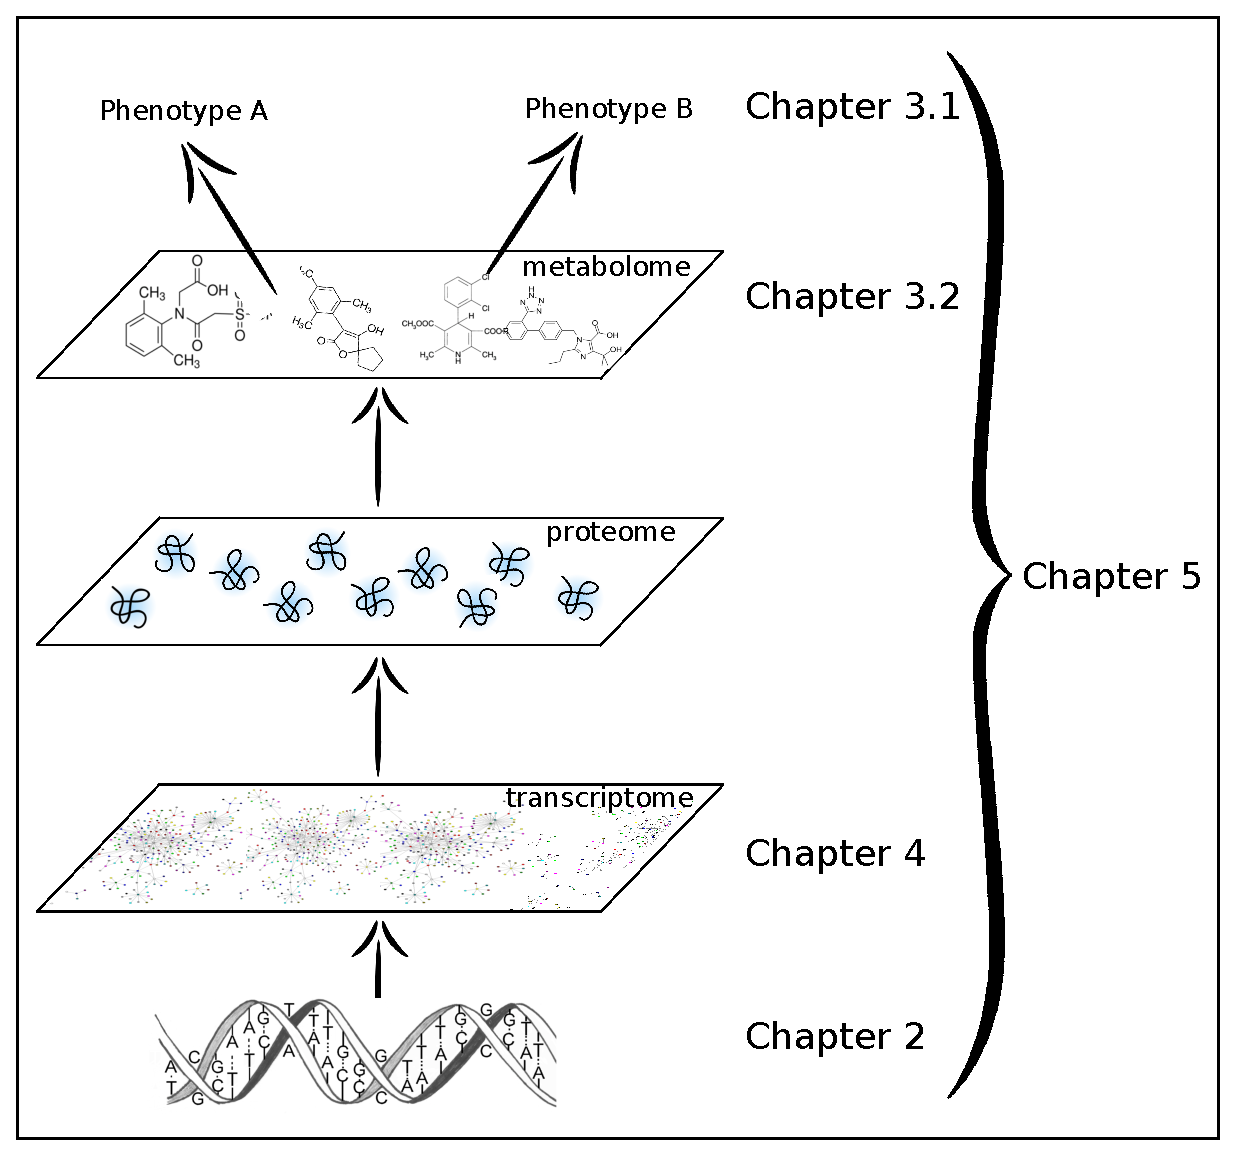
\includegraphics[width=0.6\textwidth]{eps/image_1_3}
%  \caption[ThesisLayout.]
%    {Schematic figure showing to which molecular level each chapter is related. Each molecular 
%    level here depicted are drawn from genome (bottom) to phenome (top), arrows indicate 
%    how genetic information is transferred from level to the level as by the current by 
%    the biological 'dogma'.}
%    \label{fig:layout}
%\end{figure}

%\section{Thesis contributions (2010-2014)}
%This thesis advocates that using smarter more optimized algorithms such as Pheno2Geno 
%(Chapter \ref{chap:pheno2geno}) or Multiple QTL mapping (Chapter \ref{chap:mqm}), 
%combined with taking advantage of modern shared computational infrastructure can provide 
%a solution to the 'Big Data' challenge. Federated computing, and collaborative research 
%requires tools such as xQTL workbench (Chapter \ref{chap:xqtlwormbench}) to work 
%together and avoid duplicate efforts.

%The following chapters will highlight in more detail the different contributions made to 
%the field of systems genetics during the 4 years of my PHD research at the University of 
%Groningen. A schematic overview connecting chapters to the different bio molecular levels 
%can be found in Figure \ref{fig:layout}.

%Chapter \ref{chap:pheno2geno} details how Pheno2Geno an R package was developed for 
%the high-throughput generation of genetic markers and maps from molecular phenotypes. 
%Pheno2Geno selects suitable phenotypes that show clear differential expression in the founders. Pheno2Geno 
%uses mixture modeling to select phenotypes showing segregation ratios close to the 
%expected Mendelian segregation ratios and transform them into genetic markers suitable 
%for map construction and/or saturation. Pheno2Geno analyzes the candidate genetic 
%markers and excludes those showing multiple QTL, epistatically interacting QTL, and QTL 
%by environment interactions to provide a set of robust markers for QTL mapping protecting 
%against genetic markers from a non genetic origin.

%Chapter \ref{chap:mqm} highlights the integration of the Multiple QTL mapping algorithm 
%into R/qtl. In sections (\ref{chap:mqm}.1 and  \ref{chap:mqm}.2) we show the performance 
%of MQM on experimental data from a cross of \emph{A. thaliana} Bayreuth x Shahdara. We 
%focus on the developing seeds in this cross and try to find genetic factors underlying 
%changes we observed in the phenome and metabolome.

%Chapter \ref{chap:ctlmapping} -  Shows our current work on understanding differences in 
%correlation observed when mapping two traits onto the genome. We show that there is a high 
%overlap between CTL mapping and using an G:E interaction model, and apply this interaction 
%model to data from a human genome wide association study (GWAS). We detect cell type specific 
%eQTL in whole blood for neutrophils, and show that low effect QTLs observed in samples can be explained by 
%compensating for the relative number of neutrophils observed, or predicted. Cell type specific 
%eQTL analysis will improving our power to detect QTLs and enables us to assign cell type labels 
%to observed \emph{cis}-eQTL effects.

%Chapter \ref{chap:xqtlwormbench} - Details our work to provide infrastructure for the Life 
%Sciences. We advocate the use of Generators to create software and propose a data model (XGAP) 
%to store phenotype and genotype data. Combining these two approaches we developed: xQTL 
%workbench a scalable web platform for the mapping of quantitative trait loci (QTLs) at 
%multiple levels such as gene expression (eQTL), protein abundance (pQTL), metabolite 
%abundance (mQTL) and phenotype (phQTL) data. Popular QTL mapping methods for model organism 
%and human populations are accessible via the web user interface. Large calculations scale %
%easily on to multi-core computers, clusters and cloud computing.

%There are enough subjects to cover in this thesis. We start by improving the genetic map for 
%our model organism \emph{A. thaliana}. We introduce Multiple QTL mapping (MQM), which we use 
%to find genetic loci involved in seed quality traits in \emph{A. thaliana}. We expand our 
%methodology by looking at different environments and realize cell type is just another 
%factors which can be handled in a similar way as environments. Finally we discuss the 
%implications of the ever increasing stream of raw data available through new technologies and 
%our vision (xQTL workbench) on how to handle big data and avoid duplicated effort by a 
%collaborative research platform.

